\section{Die $\Gamma$-Funktion im Kugelvolumen\label{gamma:section:teil0}}
\kopfrechts{$\Gamma$ in Kugelvolumen}
Da wir jetzt die $\Gamma$-Funktion kennen, können wir die Formel~\eqref{gamma-eq:n-sphere-volume-even} 
zur Berechnung des Kugelvolumens erweitern und alle Kugelvolumina mit
\begin{equation}
\label{gamma-eq:n-sphere-volume}
    V_n(r) = \frac{\pi^{n/2}}{\Gamma(\frac{n}{2}+1)}  r^n
\end{equation}
berechnen. 
Somit ist es nun auch möglich Kugelvolumina ungerader Dimensionen zu bestimmen.
Wir erfahren zum Beispiel, dass das Volumen einer $1$-dimensionalen Einheitskugel $V_1(1) = 2$ sein muss. 
Intuitiv ist das sinnvoll, wie Abb.~\ref{gamma-fig:1-dim-sphere} zeigt.

\begin{figure}
    \centering
    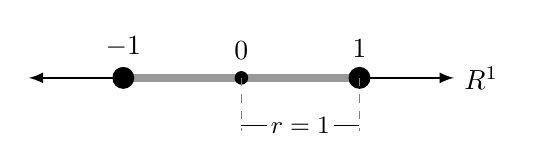
\begin{tikzpicture}[scale=1.5]
        \draw[latex-latex, thick, black] (-1.8, 0) -- (1.8, 0) node[right, black] {$\mathbb{R}^1$};
        \draw[line width=1mm, gray!80, cap=round] (-1, 0) -- (1, 0);
        \filldraw[black] (0,0) circle (1.5pt) node[above=3pt] {$0$};
        \filldraw[black] (-1,0) circle (2.5pt) node[above=4pt] {$-1$};
        \filldraw[black] (1,0) circle (2.5pt) node[above=4pt] {$1$};
        \draw[dimen/.style={<->, >=Latex, blue, thin}]
            (0, -0.4) -- node[fill=white, inner sep=1.5pt, font=\small] {$r = 1$} (1, -0.4);
        \draw[gray, dashed] (0, 0) -- (0, -0.45);
        \draw[gray, dashed] (1, 0) -- (1, -0.45);
    \end{tikzpicture}
    \caption{Die $1$-dimensionale Einheitskugel.}
    \label{gamma-fig:1-dim-sphere}
\end{figure}

Dieses Resultat hat die interessante Konsequenz, dass $\Gamma(\frac{3}{2}) = \frac{1}{2} \sqrt{\pi}$, weil sie $\sqrt{\pi}$ im Zähler ausgleichen muss.
